\sectionold{\StructurePackingSectionName}
\label{structure_packing}

Достаточно немаловажный момент, это упаковка полей в структурах\footnote{См. также: \URLWPDA}.

Возьмем простой пример:

\lstinputlisting{patterns/15_structs/4_packing/packing.c}

Как видно, мы имеем два поля \Tchar (занимающий один байт) и еще два ~--- \Tint (по 4 байта).

% subsections:
\subsection{x86}

Компилируется это все в:

\lstinputlisting[caption=MSVC 2012 /GS- /Ob0,label=src:struct_packing_4,numbers=left]{patterns/15_structs/4_packing/packing_RU.asm}

Кстати, мы передаем всю структуру, но в реальности, как видно, структура в начале копируется
во временную структуру (выделение места под нее в стеке происходит в строке 10,
а все 4 поля, по одному, копируются в строках 12 \ldots\ 19), 
затем передается только указатель на нее (или адрес).

Структура копируется, потому что неизвестно, будет ли функция \ttf модифицировать структуру или нет.
И если да, то структура внутри \main должна остаться той же.

Мы могли бы использовать указатели на \CCpp, и итоговый код был бы почти такой же,
только копирования не было бы.

Мы видим здесь что адрес каждого поля в структуре выравнивается по 4-байтной границе. 
Так что каждый \Tchar здесь занимает те же 4 байта что и \Tint. Зачем? 
Затем что процессору удобнее обращаться по таким адресам и кэшировать данные из памяти.

Но это не экономично по размеру данных.

Попробуем скомпилировать тот же исходник с опцией (\TT{/Zp1}) 
(\IT{/Zp[n] pack structures on n-byte boundary}).

\lstinputlisting[caption=MSVC 2012 /GS- /Zp1,label=src:struct_packing_1,numbers=left]
{patterns/15_structs/4_packing/packing_msvc_Zp1_RU.asm}

Теперь структура занимает 10 байт и все \Tchar занимают по байту. Что это дает? 
Экономию места. Недостаток ~--- процессор будет обращаться к этим полям не так эффективно 
по скорости, как мог бы.

\label{short_struct_copying_using_MOV}
Структура так же копируется в \main. Но не по одному полю, а 10 байт, при помощи трех
пар \MOV.

Почему не 4?
Компилятор рассудил, что будет лучше скопировать 10 байт
при помощи 3 пар \MOV, чем копировать два 32-битных слова и два байта при помощи 4 пар \MOV.

Кстати, подобная реализация копирования при помощи \MOV взамен вызова функции \TT{memcpy()}, например, это
очень распространенная практика, потому что это в любом случае работает быстрее чем вызов \TT{memcpy()} ---
если речь идет о коротких блоках, конечно: \myref{copying_short_blocks}.

Как нетрудно догадаться, если структура используется много в каких исходниках и объектных файлах, 
все они должны быть откомпилированы с одним и тем же соглашением об упаковке структур.

\newcommand{\FNURLMSDNZP}{\footnote{\href{http://go.yurichev.com/17067}
{MSDN: Working with Packing Structures}}}
\newcommand{\FNURLGCCPC}{\footnote{\href{http://go.yurichev.com/17068}
{Structure-Packing Pragmas}}}

Помимо ключа MSVC \TT{/Zp}, указывающего, по какой границе упаковывать поля структур, есть также 
опция компилятора \TT{\#pragma pack}, её можно указывать прямо в исходнике. 
Это справедливо и для MSVC\FNURLMSDNZP и GCC\FNURLGCCPC{}.

Давайте теперь вернемся к \TT{SYSTEMTIME}, которая состоит из 16-битных полей. 
Откуда наш компилятор знает что их надо паковать по однобайтной границе?

В файле \TT{WinNT.h} попадается такое:

\begin{lstlisting}[caption=WinNT.h]
#include "pshpack1.h"
\end{lstlisting}

И такое:

\begin{lstlisting}[caption=WinNT.h]
#include "pshpack4.h"                   // 4 byte packing is the default
\end{lstlisting}

Сам файл PshPack1.h выглядит так:

\begin{lstlisting}[caption=PshPack1.h]
#if ! (defined(lint) || defined(RC_INVOKED))
#if ( _MSC_VER >= 800 && !defined(_M_I86)) || defined(_PUSHPOP_SUPPORTED)
#pragma warning(disable:4103)
#if !(defined( MIDL_PASS )) || defined( __midl )
#pragma pack(push,1)
#else
#pragma pack(1)
#endif
#else
#pragma pack(1)
#endif
#endif /* ! (defined(lint) || defined(RC_INVOKED)) */
\end{lstlisting}

Собственно, так и задается компилятору, как паковать объявленные после \TT{\#pragma pack} структуры.

\clearpage
\subsubsectionold{\olly + упаковка полей по умолчанию}
\myindex{\olly}

Попробуем в \olly наш пример, где поля выровнены по умолчанию (4 байта):

\begin{figure}[H]
\centering
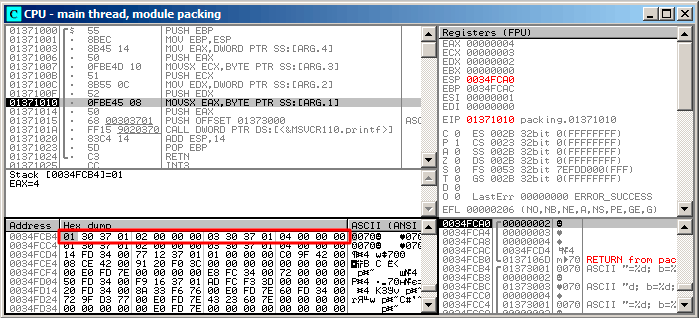
\includegraphics[scale=\FigScale]{patterns/15_structs/4_packing/olly_packing_4.png}
\caption{\olly: Перед исполнением \printf}
\label{fig:packing_olly_4}
\end{figure}

В окне данных видим наши четыре поля.
Вот только, откуда взялись случайные байты (0x30, 0x37, 0x01) рядом с первым (a) и третьим (c) полем?

Если вернетесь к листингу \myref{src:struct_packing_4}, то увидите, что первое и третье поле имеет
тип \Tchar, а следовательно, туда записывается только один байт, 1 и 3 соответственно (строки 6 и 8).

Остальные три байта 32-битного слова не будут модифицироваться в памяти!

А, следовательно, там остается случайный мусор.
\myindex{x86!\Instructions!MOVSX}
Этот мусор никак не будет влиять на работу \printf,
потому что значения для нее готовятся при помощи инструкции \MOVSX, которая загружает
из памяти байты а не слова: 
\lstref{src:struct_packing_4} (строки 34 и 38).

Кстати, здесь используется именно \MOVSX (расширяющая знак), потому что тип 
\Tchar --- знаковый по умолчанию в MSVC и GCC.

Если бы здесь был тип \TT{unsigned char} или \TT{uint8\_t}, 
то здесь была бы инструкция \MOVZX.

\clearpage
\subsubsectionold{\olly + упаковка полей по границе в 1 байт}
\myindex{\olly}

Здесь всё куда понятнее: 4 поля занимают 10 байт и значения сложены в памяти друг к другу

\begin{figure}[H]
\centering
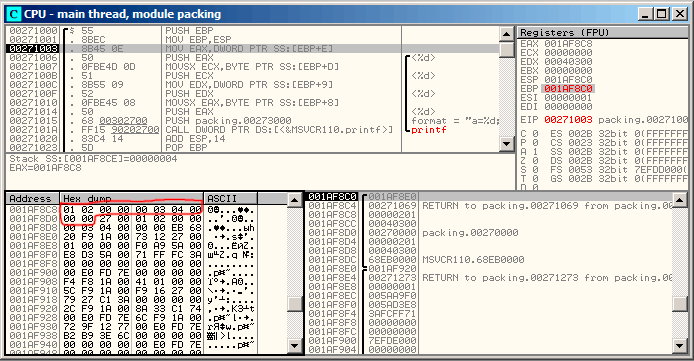
\includegraphics[scale=\FigScale]{patterns/15_structs/4_packing/olly_packing_1.png}
\caption{\olly: Перед исполнением \printf}
\label{fig:packing_olly_1}
\end{figure}


\subsection{ARM}

\subsubsection{\OptimizingKeilVI (\ThumbMode)}

\lstinputlisting[caption=\OptimizingKeilVI (\ThumbMode)]{patterns/15_structs/4_packing/packing_Keil_thumb.asm}

Как мы помним, здесь передается не указатель на структуру, а сама структура, а так как в ARM первые 4 аргумента
функции передаются через регистры, то поля структуры передаются через \TT{R0-R3}.

\myindex{ARM!\Instructions!LDRB}
\myindex{x86!\Instructions!MOVSX}
Инструкция \TT{LDRB} загружает один байт из памяти и расширяет до 32-бит учитывая знак.

Это то же что и инструкция \MOVSX в x86.
Она здесь применяется для загрузки полей $a$ и $c$ из структуры.

\myindex{Function epilogue}
Еще что бросается в глаза, так это то что вместо эпилога функции, переход на эпилог другой функции!

Действительно, то была совсем другая, не относящаяся к этой, функция, однако, она имела точно такой же эпилог 
(видимо, тоже хранила в стеке 5 локальных переменных ($5*4=0x14$)).
К тому же, она находится рядом (обратите внимание на адреса).

Действительно, нет никакой разницы, какой эпилог исполнять, если он работает так же, как нам нужно.

Keil решил использовать часть другой функции, вероятно, из-за экономии.

Эпилог занимает 4 байта, а переход ~--- только 2.

\subsubsection{ARM + \OptimizingXcodeIV (\ThumbTwoMode)}

\lstinputlisting[caption=\OptimizingXcodeIV (\ThumbTwoMode)]{patterns/15_structs/4_packing/packing_Xcode_thumb.asm}

\myindex{ARM!\Instructions!SXTB}
\myindex{x86!\Instructions!MOVSX}
\TT{SXTB} (\IT{Signed Extend Byte}) это также аналог \MOVSX в x86.
Всё остальное ~--- так же.


\subsection{MIPS}
\label{MIPS_structure_big_endian}

\lstinputlisting[caption=\Optimizing GCC 4.4.5 (IDA),numbers=left]{patterns/15_structs/4_packing/MIPS_O3_IDA.lst}

Поля структуры приходят в регистрах \$A0..\$A3 и затем перетасовываются в регистры \$A1..\$A4 для \printf.

Но здесь есть две инструкции SRA (\q{Shift Word Right Arithmetic}), которые готовят поля типа \Tchar.

Почему?
По умолчанию, MIPS это big-endian архитектура \myref{sec:endianness}, и Debian Linux в котором мы работаем, также big-endian.

Так что когда один байт расположен в 32-битном элементе структуры, он занимает биты 31..24.

И когда переменную типа \Tchar нужно расширить до 32-битного значения, она должна быть сдвинута вправо
на 24 бита.

\Tchar это знаковый тип, так что здесь нужно использовать арифметический сдвиг вместо логического.



\subsectionold{Еще кое-что}

Передача структуры как аргумент функции (вместо передачи указателя на структуру) это то же
что и передача всех полей структуры по одному.

Если поля в структуре пакуются по умолчанию, то функцию f() можно переписать так:

\begin{lstlisting}
void f(char a, int b, char c, int d)
{
    printf ("a=%d; b=%d; c=%d; d=%d\n", a, b, c, d);
};
\end{lstlisting}

И в итоге будет такой же код.
